\section{Random walks and diffusion-based methods}
\label{sec:ch10:diffusion}

Although this book puts a heavy emphasis on spectral methods, there are many ways in which we can learn lower-dimensional representations for networks which don't involve spectral approaches. As opposed to spectral methods, a \textit{random walk on a network} is a random process which focuses on the analysis of paths which start at a node in the network, and proceed to generate successions of random steps to other nodes in the network. The manner in which these random processes materialize is a function of the topology of the random network, including the nodes, edges, and (optionally, if the network is weighted), the edge weights. 
\subsection{A simplified first-order random walk on a network}

For instance, let's consider an extremely simplified approach for a first-order random walk on the network that we saw back in Section \ref{sec:ch4:prop-net}, which was the New York Bridge example. To begin, let's redefine the nodes and edges of the network. The nodes of the network are the five boroughs of New York City (Staten Island SI, Brooklyn BK, Queens Q, the Bronx BX, and Manhattan MH). The nodes in our network are the five boroughs. The edges $(i,j)$ of our network exist if one can travel from borough $i$ to borough $j$ along a bridge.

To get us started, let's take a look back at the example data that we were using:

\begin{lstlisting}[style=python]
import numpy as np

# define the node names
node_names = ["SI", "MH", "BK", "Q", "BX"]
# define the adjacency matrix
A = np.array([[0,0,1,0,0],  # staten island is neighbors of brooklyn
              [0,0,1,1,1],  # manhattan is neighbors of all but staten island
              [1,1,0,0,0],  # brooklyn is neighbors of staten island and manhattan
              [0,1,0,0,1],  # queens is neighbors of manhattan and bronx
              [0,1,0,1,0]]) # bronx is neighbors of manhattan and queens
\end{lstlisting}

We showed this network as a layout plot and an adjacency matrix in Figure \ref{fig:ch4:nyc_ex}, which you can take a look back at to refamiliarize yourself with the network.

We will imagine that there is a conference we are attending in Manhattan in Manhattan, and we decide to explore the city somewhat randomly. When we are in a given borough $i$, we will determine the next borough to explore by letting random chance do the work for us. To better define a first-order random walk, we need to introduce a background concept first: the Markov chain and the Markov property. 

\subsubsection*{Markov chains and the markov property}

A \textit{finite-space markov chain} is a model of a random system in which we have a sequence of possible events which can occur which are finite (the boroughs we will visit on a day $t$) in which the probability of each event depends only on the event in which we were previously. For network analysis, we only need to think about finite-space Markov chains, because the network has a finite collection of possible events which can occur (the nodes in the network being visited). To put this down quantitatively, the markov chain is represented by the sequence $\mathbf s_0, \mathbf s_1, \mathbf s_2, ...$, where each $\mathbf s_t$ takes the value of one of the $n$ total nodes in the network. 

You will notice that in our definition of the finite-space markov chain, we made a disclaimer: the probability of each event depends only on the state in which we were previously. This is called the \textit{markov property}. The idea is that, if we were in Manhattan at the previous step in time $t - 1$ (e.g., $\mathbf s_{t-1}$ realized the value $v_{MH}$, or $\mathbf s_{t-1} = v_{MH}$ for short), that if our current step in the Markov Chain were Brooklyn ($\mathbf s_t = v_{BK}$), that the next step in the Markov chain would not depend at all on the fact that we already saw Manhattan. 

\paragraph*{First-order random walks on a network as a markov chain}

To exhibit the ideas of a markov chain, we will define a first-order random walk on our New York Boroughs. Remember that the borough we are at, $i$, has $d_i$ possible neighboring boroughs, where $d_i$ was the degree of node $i$. You will visit one of the other nodes in the network as follows. If borough $j$ is a neighbor of borough $i$ (an edge exists from borough $i$ to borough $j$), we will visit borough $j$ with probability $\frac{1}{d_i}$. The idea is that we will visit neighbors of each borough at random, depending only on whether we can get to that borough along an edge of the network. This is called a \textit{first-order random walk} because it is a random walk where we ignore everything about the path we have taken to get to our current borough to date, except for the fact that we are at that borough now. This means that our next borough will not depend at all on whether we have already been to that borough in our exploration of the city. If the node is not a neighbor of our current borough, we will visit it with probability $0$. 

Stated another way, if we are in node $i$ at time $t$ (that is, $s_t = i$), the probability of going to another node $j$ is defined as:
\begin{align*}
    p_{ij} &= \begin{cases}
        \frac{1}{d_i},  & \text{edge $(i,j)$ exists} \\
        0,  & \text{edge $(i,j)$ does not exist}
    \end{cases}\numberthis \label{eqn:next:diff:trans_mtx}
\end{align*}
Note that these probabilities, called the \textit{transition probability} from node $i$ to node $j$, do not have anything to do with which nodes we have visited yet, and these transition probabilities are always the same. For this reason, while we could have used the notation $p_{ij}^{(t+1)}$ in place of $p_{ij}$, we will avoid doing so (because it is confusing). 

Further, since these probabilities are unchanging in time, they are often organized into an $n \times n$ matrix, called the \textit{transition probability matrix} $P$ with entries $p_{ij}$ defined as above. In this case, the transition probability matrix can be arranged like this:

\begin{lstlisting}[style=python]
# compute the degree of each node
di = A.sum(axis=0)
# the probability matrix is the adjacency divided by
# degree of the starting node
P = (A / di).T
\end{lstlisting}

The transition probability matrix is illustrated in a heatmap in Figure \ref{fig:next:diff:trans_mtx}(B), with the corresponding layout plot for the network in  Figure \ref{fig:next:diff:trans_mtx}(A). Notice that if we are in Staten Island, there is only one borough we can go from here, so with probability $1$, we will visit its only neighbor: Brooklyn. If we are in Manhattan, we could go to any of its three neighbors (Brooklyn, Queens, or Bronx), with equal probability $\frac{1}{3}$. If we were in Brooklyn, we could visit any of its two neighbors (Manhattan or Staten Island) with equal probability $\frac{1}{2}$. This continues for each node in the network until we have successfully generated the transition probability matrix $P$. Note further that since the transition probability entries $p_{ij}$ are normalized only by the degree $d_i$ of the node $i$, the transition probability matrix is not necessarily symmetric, even if the network is undirected (and has a symmetric adjacency matrix). 

\begin{figure}
    \centering
    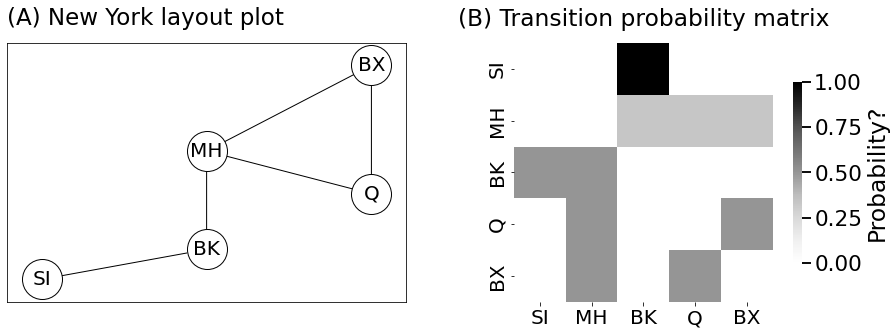
\includegraphics[width=0.8\linewidth]{next/Images/first_ord.png}
    \caption[Transition probability matrix for the network]{\textbf{(A)} the New York bridge network, and \textbf{(B)} the transition probability matrix for the network.}
    \label{fig:next:diff:trans_mtx}
\end{figure}

There are a lot of interesting properties we can use the transition probability matrix $P$ to learn about, but we will not cover them all here. If you want some more details on transition probability matrices and Markov chains in general, we would recommend that you check out a book on stochastic processes, such as our favorite \cite{Isaacson1976Mar}.

Next, let's use this transition probability matrix to generate a random walk on the New York City boroughs. As we mentioned, our hotel is in Manhattan, so we are going to start our random walk through the city here. In Figure \ref{fig:next:diff:step}(A), we illustrate a starting node, MH, in black. In other words, $\mathbf s_0 = v_{MH}$. For our next step in the Markov chain, we will visit either Brooklyn, Bronx, or Queens with probability $\frac{1}{3}$, or Staten Island with probability $0$. The nodes with non-zero transition probabilities are illustrated in dark gray, and are connected to $MH$ via edges, shown in dark black. Staten Island is inaccessible directly from MH, and is in white. The corresponding transition probabilities for each of the nodes in the network are highlighted in Figure \ref{fig:next:diff:step}(B). 

\begin{figure}
    \centering
    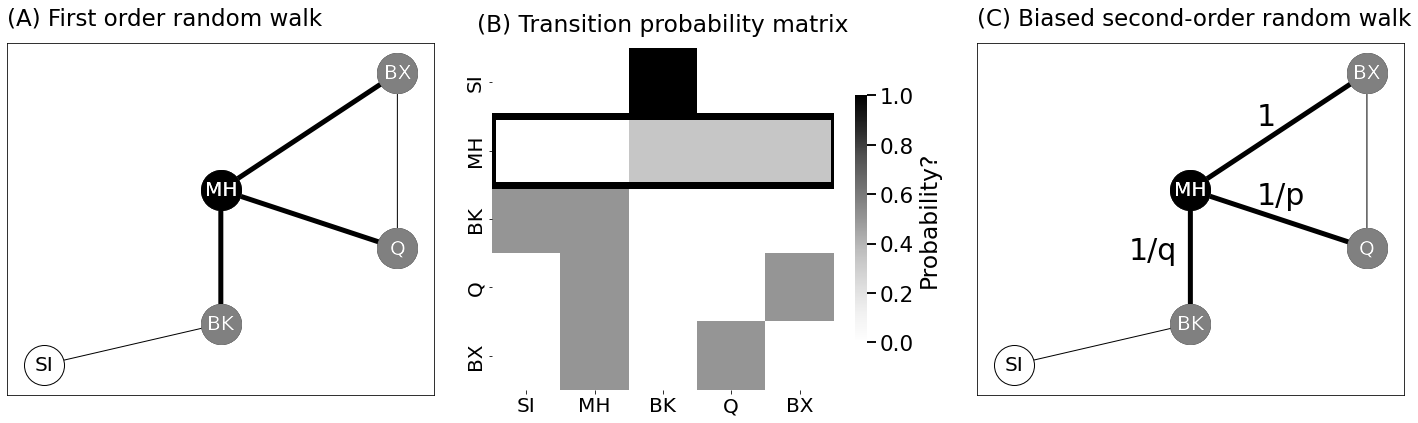
\includegraphics[width=\linewidth]{next/Images/one_step.png}
    \caption[A transition step from MH]{\textbf{(A)} The possible next nodes that can be accessed from MH, \textbf{(B)} their corresponding probabilities, \textbf{(C)} the bias vectors for a biased second-order random walk.}
    \label{fig:next:diff:step}
\end{figure}

We then choose the next node to visit using these transition probabilities, by generating the probability vector of the next step in the random walk given the current step. We will denote this probability vector with the symbol $\vec p_i$, which is the probability vector for which node we will visit at the next step given that we are currently at node $i$. Again here we could have used the notation $\vec p_i^{(t + 1)}$ since it is the probability vector where $s_t = i$ for the $t+1$ step, but we will avoid it to keep the notation as simple as possible.

Notice that this is just the entries of the $i^{th}$ row of the transition probability matrix, which can be calculated using the relationship:
\begin{align*}
    \vec p_i &= P^\top \vec x^{(i)}
\end{align*}
where $\vec x^{(i)}$ is the vector which has a value of $0$ for all entries except for entry $i$, where it has a value of $1$. This ends up pulling out the $i^{th}$ row of $P$, because every multiplication except for those against the $i^{th}$ column of $P^\top$ (which is the $i^{th}$ row of $P$, by definition of a transpose) will end up just being $0$. Let's break it down step-by-step:
\begin{align*}
    \vec p_i &= \begin{bmatrix}
    p_{11} & ... & p_{1n} \\
    \vdots & \ddots & \vdots \\
    p_{n1} & ... & p_{nn}
    \end{bmatrix}^\top\vec x^{(i)} \\
     &= \begin{bmatrix}
    p_{11} & ... & p_{n1} \\
    \vdots & \ddots & \vdots \\
    p_{1n} & ... & p_{nn}
    \end{bmatrix}\vec x^{(i)},
\end{align*}
Where in the above step, we just transposed $P$. Using the definition of matrix multiplication gives us:
\begin{align*}
    &= \begin{bmatrix}
        p_{11}x_{1}^{(i)} + p_{21} x_2^{(i)} + ... p_{n1}x_n^{(i)} \\
        \vdots \\
        p_{1n}x_{1}^{(i)} + p_{2n} x_2^{(i)} + ... p_{nn}x_n^{(i)} 
    \end{bmatrix}, \\
    &= \begin{bmatrix}
        p_{i1} \\
        \vdots \\
        p_{in}
    \end{bmatrix}
\end{align*}
where the last step in the multiplication is because $x_{i}^{(i)}$ is the only entry which has a value of $1$, so all of the other multipilications are just $0$. 

We can pick the next node easily by just using \texttt{numpy}:

\begin{lstlisting}[style=python]
x0 = np.array([0,1,0,0,0])  # x vector indicating we start at MH
p1 = P.T @ x0  # p vector for timestep 1 starting at node MH at time 0
# choose the next node using the probability vector we calculated
next_node = np.random.choice(range(0, len(node_names)), p=p1)
print("Next node: {:s}".format(node_names[next_node]))
\end{lstlisting}


This gives us a realization of $\mathbf s_1$ as the indicated node in the network, conditional on the starting node being $\mathbf s_0 = v_{MH}$. We can generate a $T$-step first-order random walk along the network $G$ by repeating this approach, as explained in Algorithm \ref{alg:next:diff:first_ord_rw}.

\begin{algorithm}
\label{alg:next:diff:first_ord_rw}
\caption{First order random walk on a network}
\KwData{$A$ the adjacency matrix for an $n$-node network. \newline
$s_0$ the index of the node from which the random walk will begin. \newline
$T$ the number of steps to take in the random walk.
}
\KwResult{$\vec s = (s_0, s_1, \hdots, s_T)$ is a length $T+1$ vector, defining the nodes of the random walk on the network.}
\SetAlgoLined

Construct the degree matrix for the network, $D$, and let $P$ be defined as described in Equation \eqref{eqn:next:diff:trans_mtx}.


Initialize $\vec x^{(s_0)}$ to be the length $n$ vector where $x_{s_0}^{(s_{0})} = 1$, and $0$ otherwise.

\For{$t$ in $1:T$}{
    Construct a vector $\vec p_{s_{t - 1}} = P^\top \vec x^{(s_{t - 1})}$.

    Obtain a $n$-sided die, where the probability of landing on side $j$ is $p_{s_{t - 1}j}$.

    Roll the die, and let $s_t$ be the side that the die lands on.

    Let $\vec x^{(s_{t})}$ be the vector where $x_{s_t}^{(s_{t})} = 1$, and $0$ otherwise.
}

\Return{$\vec s$.}
\end{algorithm}


\subsection{What do markov chains and random walks have to do with embedding networks?}

In the preface for this section, we said we were going to cover how to use a random walk to embed our network, but we've ignored that thus far. To get us to what this has to do with embeddings, we need to introduce a slight variation of the random walk we developed in the preceding section, called the second-order biased random walk.
\subsubsection*{Second-order biased random walk}

Remember when we developed our first-order random walk, we did something kind of nonsensical: we ignored all of the previous boroughs of New York we had already seen, and said that the next borough was only a function of the current borough we are at. You could certainly imagine that we get caught in a legitimate random walk (it is a possible realization because all of the transition probabilities are positive) where we explore going from Manhattan to Brooklyn, and then over to Staten Island, and then back to Brooklyn, and then back to Staten Island, so on and so forth, because we totally ignored the previous places we had been when making our decision for where to go from our current borough. 

If we are tourists trying to explore New York, we obviously will want to get a better sense of all of the city, and want to favor the boroughs we haven't been to as recently. In the second-order biased random walk, we introduce the idea of the return and in-out parameters, $p$ and $q$, respectively. 

\paragraph*{The bias factor lets us control our ability to leave or remain amongst a neighborhood of nodes}

Remember that the steps in our random walk, $\left\{\mathbf s_0, \mathbf s_1, ..., \mathbf s_{t-1}, \mathbf s_t, ...\right\}$, were sequences of random variables which took values of our nodes in the network. Let's assume that we have a random walk so far, where at our previous state, $\mathbf s_{t-1} = s_{t-1}$, and we are currently at node $i$, $\mathbf s_t = i$. Here, $s_{t-1}$ is some other node which we just came from to get to node $i$.

The \textit{in-out} parameter $q$ is a value which indicates a bias factor of $\frac{1}{q}$ that we will go to some node $j$ that is totally disconnected from the previous node that we visited, $s_{t-1}$. This means that in our network, there is no edge starting at node $j$ and going to node $s_{t-1}$. If the in-out parameter $q$ takes big values, then $\frac{1}{q}$ will be very small, and we will be biased against visiting nodes which are not connected to the previous node we visited. If $q$ is small, then $\frac{1}{q}$ will be very big, and we will be biased towards visiting nodes which are not connected to the previous node we visited. In other words, high in-out parameters get us ``out'' of nodes connected to those we just visited.

The \textit{return} parameter $p$ is a value which indicates a bias factor of $\frac{1}{p}$ that we will go back to the node which we visited previously in the last state $s_{t-1}$. If the return parameter $p$ takes big values, $\frac{1}{p}$ will be very small, and we will be biased against visiting a node we have just been to. If $p$ is small, then $\frac{1}{p}$ will be very big, and we will be biased towards visiting a node which we were just at. In other words, a high return parameter $p$ ``returns'' us to the node we just visited.

If a node satisfies neither of these conditions, the bias factor is just left at $1$. Together, these relationships are summarized with the \textit{second-order bias factors} $\alpha_{ij}(p,q, s_{t-1})$ starting at node $s_t = i$ and proceeding to node $j$ with parameters $p$ and $q$ for the next step $t+1$ given that we just left state $s_{t-1}$ as:
\begin{align*}
    \alpha_{ij}(p,q,s_{t-1}) &= \begin{cases}
        \frac{1}{p}, & \text{$s_{t-1} = j$} \\
        \frac{1}{q}, & \text{$s_{t-1} \neq j$ and the edge $(j,s_{t-1})$ exists} \\
        1, & \text{$s_{t-1} \neq j$ and no edge $(j,s_{t-1})$ exists}
    \end{cases}\numberthis \label{eqn:next:diff:bias}
\end{align*}
The corresponding second-order bias vector is $\vec \alpha_{i}(p,q, s_{t-1})$, which is a vector of each of the bias factors for all of the other $n$ nodes in the network. These are called second-order because they depend on the current node, $i$, as well as the preceding node, $s_{t-1}$.

Let's work this up with an example, in Figure \ref{fig:next:diff:step}(C). We'll consider a biased second-order random walk, where the current node we are on is Manhattan ($s_t = v_{MH}$) and is shown in black, and the previous node we visited was Queens ($s_{t-1} = v_{Q}$) and is shown in light gray. We just visited node $Q$, so the bias factor will be $\frac{1}{p}$. The node for Brooklyn does not have an edge back to Queens, so taking it gets us ``out'', and the bias factor will be $\frac{1}{q}$. The node for Bronx does has an edge back to queens, so the bias is $1$.

If we were to tend to bias against returning (a large return parameter, say $p = 5$) and towards in-out (a small in-out parameter, say $q = \frac{1}{2}$), we can do it like this:

\begin{lstlisting}[style=python]
p = 5  # return parameter
q = 1/2  # in-out parameter
bias_vector = np.ones(len(node_names))
bias_vector[node_names == "Q"] = 1/p
bias_vector[node_names == "BK"] = 1/q
\end{lstlisting}

The resulting bias vector is shown in Figure \ref{fig:next:diff:biased_vecs}(A). 

\begin{figure}
    \centering
    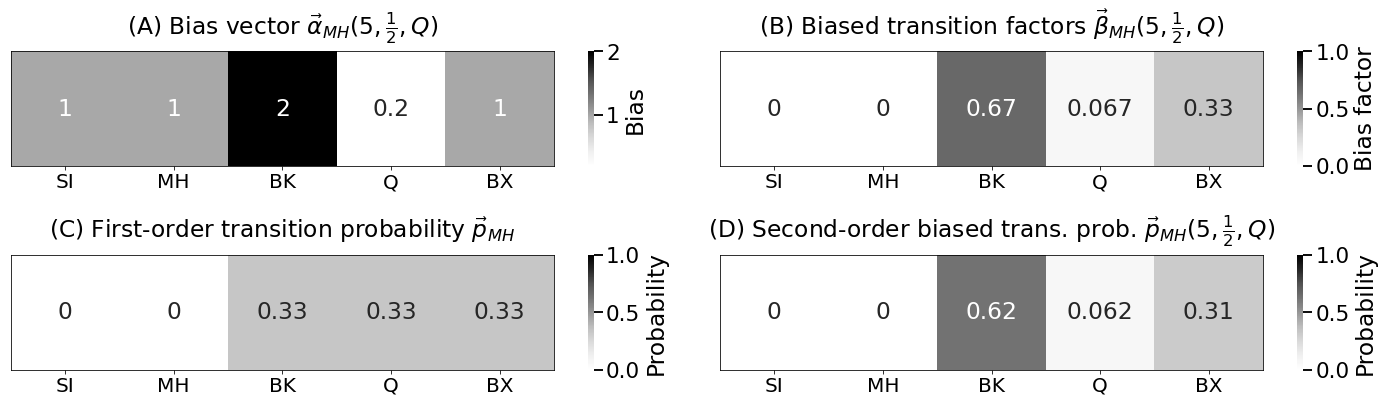
\includegraphics[width=\linewidth]{next/Images/trans_vecs.png}
    \caption[Biased second-order random walk transition probability]{With  with $p=5$ and $q = \frac{1}{2}$ for $n=5$ where $s_t = MH$ and $s_{t - 1} = Q$, \textbf{(A)} the bias vector, \textbf{(B)} the second order biased transition factors, \textbf{(C)} the first order transition probabilities, and \textbf{(D)} the second-order biased transition probabilities.}
    \label{fig:next:diff:biased_vecs}
\end{figure}

\paragraph*{Adjusting the transition probabilities with the bias vector}

In our second order random walk, instead of the transition probabilities being a function only of the current state, they are also a function of the preceding state we were at $s_{t-1}$. This means that our transition probability matrix is going to look different based on which node we just came from. The transition probabilities will be defined using the notation $p_{ij}(p,q,s_{t-1})$, where $s_{t-1}$ is the preceding node we visited, $i$ is the current node we are at, $j$ is any other node in the network, and $p$ and $q$ are the return and in-out parameters respectively. 

The first terms to define are the \textit{second-order biased transition factors}:
\begin{align*}
    \beta_{ij}(p,q, s_{t-1}) &= \alpha_{ij}(p, q, s_{t-1})p_{ij} \numberthis \label{eqn:next:diff:bias_factor}
\end{align*}
where $p_{ij}$ are the first-order markov transition probabilities we used previously. The idea here is that the biased transition factor combine the bias factor with the transition probability from the first-order markov chain.

In effect, what this statement says is that we up or down-weight (or don't change it at all, if the bias factor is $1$) the transition probability $p_{ij}$ of going from node $i$ to node $j$ based on the bias factor $\alpha_{ij}(p, q, s_{t-1})$. These are no longer probabilities, because starting at a node $i$, we might end up with the bias-adjusted transition factors no longer summing to one. This is because we did not require anything about how $\alpha_{ij}(p,q,s_{t-1})$ behaved across all possible nodes $j$ we could transition to from our current node $i$.

Finally, we then use the biased transition factors to compute the \textit{second-order biased transition probabilities}. These are just normalized versions of the biased transition factors, where we normalize to make sure that they all sum up to one (and hence, produce a valid transition probability from node $i$ outwards):
\begin{align*}
    p_{ij}(p,q,s_{t-1}) &= \frac{\beta_{ij}(p,q, s_{t-1})}{\sum_{j' = 1}^n\beta_{ij'}(p,q, s_{t-1})} \numberthis \label{eqn:next:diff:2ord_trans_probs}
\end{align*}
Notice that in the denominator, that we are just normalizing the biased transition factor by the sum of all the other biased transition factors from node $i$ to any other nodes $j'$ in the network. 

Next, we show how this computation works to update the transition probability vector from the Manhattan node to node $j$ given a previous node of Queens. We begin by first starting with the first-order transition probability vector $\vec p_i$:

\begin{lstlisting}[style=python]
xtminus1 = [0, 0, 0, 1, 0]  # previous step was at Q
xt = [0, 1, 0, 0, 0]  # starting vector at MH
pt = P.T @ xt  # probability vector is Pt*x
\end{lstlisting}

The next step is to compute the second-order biased transition factors:

\begin{lstlisting}[style=python]
bias_factors = pvec*bias_vector
\end{lstlisting}

Which is shown in Figure \ref{fig:next:diff:biased_vecs}(B). And finally, we normalize the bias-adjusted transition factors to obtain the second-order biased transition probabilities:

\begin{lstlisting}[style=python]
biased_pt = bias_factors/bias_factors.sum()
\end{lstlisting}

We compare the first-order transition probabilities to the second-order biased transition probabilities in Figure \ref{fig:next:diff:biased_vecs}(C) and \ref{fig:next:diff:biased_vecs}(D), respectively. As we can see, our tendency to return to Queens (since we were just there in the previous step, $s_{t-1} = v_{Q}$) has decreased from the first-order transition probability to the second-order biased transition probability, due to the fact that the return parameter is big ($p = 5$). Further, our tendency to move in-out to Brooklyn (since Brooklyn has no edges to Queens) has increased from the first-order transition probability to the second-order biased transition probability, due to the fact that the in-out parameter is small ($q = 0.2$). The transition probability for the remaining nodes, such as BX, with a bias of $1$ are less affected from the first-order to the second-order biased transition probability.

We then just use the second-order biased transition probabilities to decide where to go next, as we did before:

\begin{lstlisting}[style=python]
xt = np.array([0,1,0,0,0])  # x vector indicating we start at MH
# choose the next node using the second-order biased transition probability
next_node = np.random.choice(range(0, len(node_names)), p=biased_pvec)
print("Next node: {:s}".format(node_names[next_node]))
\end{lstlisting}

The procedure for generating a second-order biased random walk is described in Algorithm \ref{alg:next:diff:second_ord_biased_rw}. The reason that we set $T > 1$ in the algorithm is that if $T = 1$, the second-order biased random walk would just be a first-order random walk as in Algorithm \ref{alg:next:diff:first_ord_rw}, so the method would be redundant. 


\begin{algorithm}
\label{alg:next:diff:second_ord_biased_rw}
\caption{Second-order biased random walk}
\KwData{$A$ the adjacency matrix for an $n$-node network. \newline
$s_0$ the index of the node from which the random walk will begin. \newline
$T$ the number of steps to take in the random walk, where $T > 1$. \newline
$q$ the in-out parameter.\newline
$p$ the return parameter.
}
\KwResult{$\vec s = (s_0, s_1, \hdots, s_T)$ is a length $T+1$ vector, defining the nodes of the random walk on the network.}
\SetAlgoLined

Construct the degree matrix for the network, $D$, and let $P$ be defined as described in Equation \eqref{eqn:next:diff:trans_mtx}.

Perform a first-order random walk from $s_0$ to $s_1$, using the procedure in Algorithm \ref{alg:next:diff:first_ord_rw} with $T = 1$, to obtain the first-order random walk $(s_0, s_1)$.

Initialize $\vec x^{(s_1)}$ to be the length $n$ vector where $x_{s_1}^{(s_{1})} = 1$, and $0$ otherwise.

\For{$t$ in $2:T$}{
    Compute the bias vector $\vec \alpha_{s_{t - 1}}(p, q, s_{t - 2})$, using the equation described in Equation \eqref{eqn:next:diff:bias}.

    Compute the first order transition probability vector, $\vec p_{s_{t - 1}} = P^\top\vec x^{(s_{t - 1})}$.

    Compute the second-order bias factor vector $\vec{\beta}_{s_{t - 1}}(p, q, s_{t - 2})$, using Equation \eqref{eqn:next:diff:bias_factor} with the transition probability vector $\vec p_{s_{t - 1}}$.

    Normalize the second-order bias factors $\beta_{s_{t - 1}j}(p, q, s_{t - 2})$ for each node $j$ in the network, using Equation \eqref{eqn:next:diff:2ord_trans_probs} to obtain the second-order biased transition probabilities $p_{s_{t - 1}j}(p, q, s_{t - 2})$.

    Obtain a $n$-sided die, where the probability of landing on side $j$ is $p_{s_{t - 1}j}(p, q, s_{t - 2})$.

    Roll the die, and let $s_t$ be the side that the die lands on.

    Let $\vec x^{(s_{t})}$ be the length $n$ vector where $x_{s_t}^{(s_{t})} = 1$, and $0$ otherwise.
}

\Return{$\vec s$.}

\end{algorithm}

\subsection{The \texttt{word2vec} algorithm}

Now that we know about second-order biased random walks, we are ready to approach our problem at hand: leveraging random walks to produce structured embeddings. We have one final ingredient to embed our networks: the \texttt{word2vec} algorithm.

\subsubsection*{Background on \texttt{word2vec}}

The \texttt{word2vec} algorithm is a technique for natural language processing (NLP) developed in 2013 by a team of researchers at Google led by Tomas Mikolov. The algorithm takes in large collections of text data, called a corpus. The algorithm takes this corpus (collection, such as a set of sentences found in documents) of text along with a desired number of embedding dimensions $d$, and embeds every possible word in the corpus into a $d$-dimensional space such that the contexts of the words frequently used together are preserved. 

In this case, a \textit{context} refers to words which tend to convey similar meaning (they are synonyms), words which tend to precede be used together (for instance, ``learning’’ and ``intelligence’’), and many other attributes of the words. When we say ``preserved’’, what we mean is that words that have similar contexts tend to be closer together in the embedded space. This embedding can then be used for many different problems using different \textit{downstream} algorithms, in that \texttt{word2vec} can be thought of as a pre-processing step to turn the collection of words into useful $d$-dimensional representations. For instance, we might use \texttt{word2vec} before using other algorithms for things such as guessing the synonyms of words or suggesting next words for a sentence.

If you want to learn more about \texttt{word2vec} as it relates to word embeddings, we would suggest you dig up some blog posts on sites like medium, or by checking out the original papers by Mikolov and his team, of which the first can be found at \cite{Mikolov2013Jan} and the second can be found \cite{Mikolov2013Oct}.

\subsection{The \texttt{node2vec} embedding}

To begin the \texttt{node2vec} embedding \cite{Grover2016Aug}, we first look at the collection of nodes in our network. For each node, we generate a random walk of length $T$ using the given node as the starting node with parameters $(p,q)$, as we did above. This gives us a collection of random walks with disparate starting nodes in the network. We repeat this procedure a number of times $r$ for each possible starting node, to give us a set of $rn$ random walks of length $T$. 

Next, we ``pretend’’ that node indices are words, and we simply feed the collections of random walks we generated into \texttt{word2vec} algorithm as our ``corpus’’ of text along with the desired number of embedding dimensions $d$. Let's see how \texttt{word2vec} does this for us.

\subsubsection*{One-hot encoding the nodes}

The first step to using the \texttt{word2vec} algorithm is to convert each of the $n$ nodes in the network into vectors. Fortunately, we have already learned about one way to do this: the one-hot encoding, which we learned about above when discussing transition probability vectors. 

For a given node $i$, we can one-hot encode the node with the vector $\vec x^{(i)}$, which is a vector where $x^{(i)}_i = 1$, and $0$ otherwise. 

These one-hot encodings of the nodes will be the inputs to the skip-gram algorithm, which one of the procedures that \texttt{word2vec} can use to implicitly obtain node embeddings.

\subsubsection*{The Skip-Gram Algorithm}

The idea behind the skip-gram algorithm is quite simple. It uses neural networks, so we will note here that there are two different uses of the term `network': 

\begin{enumerate}
    \item the network that we want to embed nodes and edges from, which will be referred to as the ``network'', and
    \item the neural network, which we will use to learn embeddings of the nodes and edges of the original network, which will be referred to as the ``NN''.
\end{enumerate}

The skip-gram algorithm seeks to achieve a solution for the following problem: given a one-hot encoding of a node $i$ in the network, identify the probability that at a ``nearby'' position in the corpus of random walks is another node $j$, for each of the $n$ nodes in the network. We will begin by thinking about this objective.

\paragraph*{Sliding windows to generate training/testing samples}

To estimate the probability that at a ``nearby'' position in the corpus of random walks is another node $j$, for each of the $n$ nodes in the network, we generate training and testing data using a \textit{sliding window} with a fixed width $\omega$. 

In Figure \ref{fig:next:diff:sliding_window}(A), we look at the process of sliding a window over a random walk $t$ of width $\omega = 2$. The sliding window is constructed about a \textit{center} node, illustrated in white. The \textit{context} nodes are the nodes that we want the model to predict, illustrated in gray, when given the center node, illustrated in white.

\begin{figure}
    \centering
    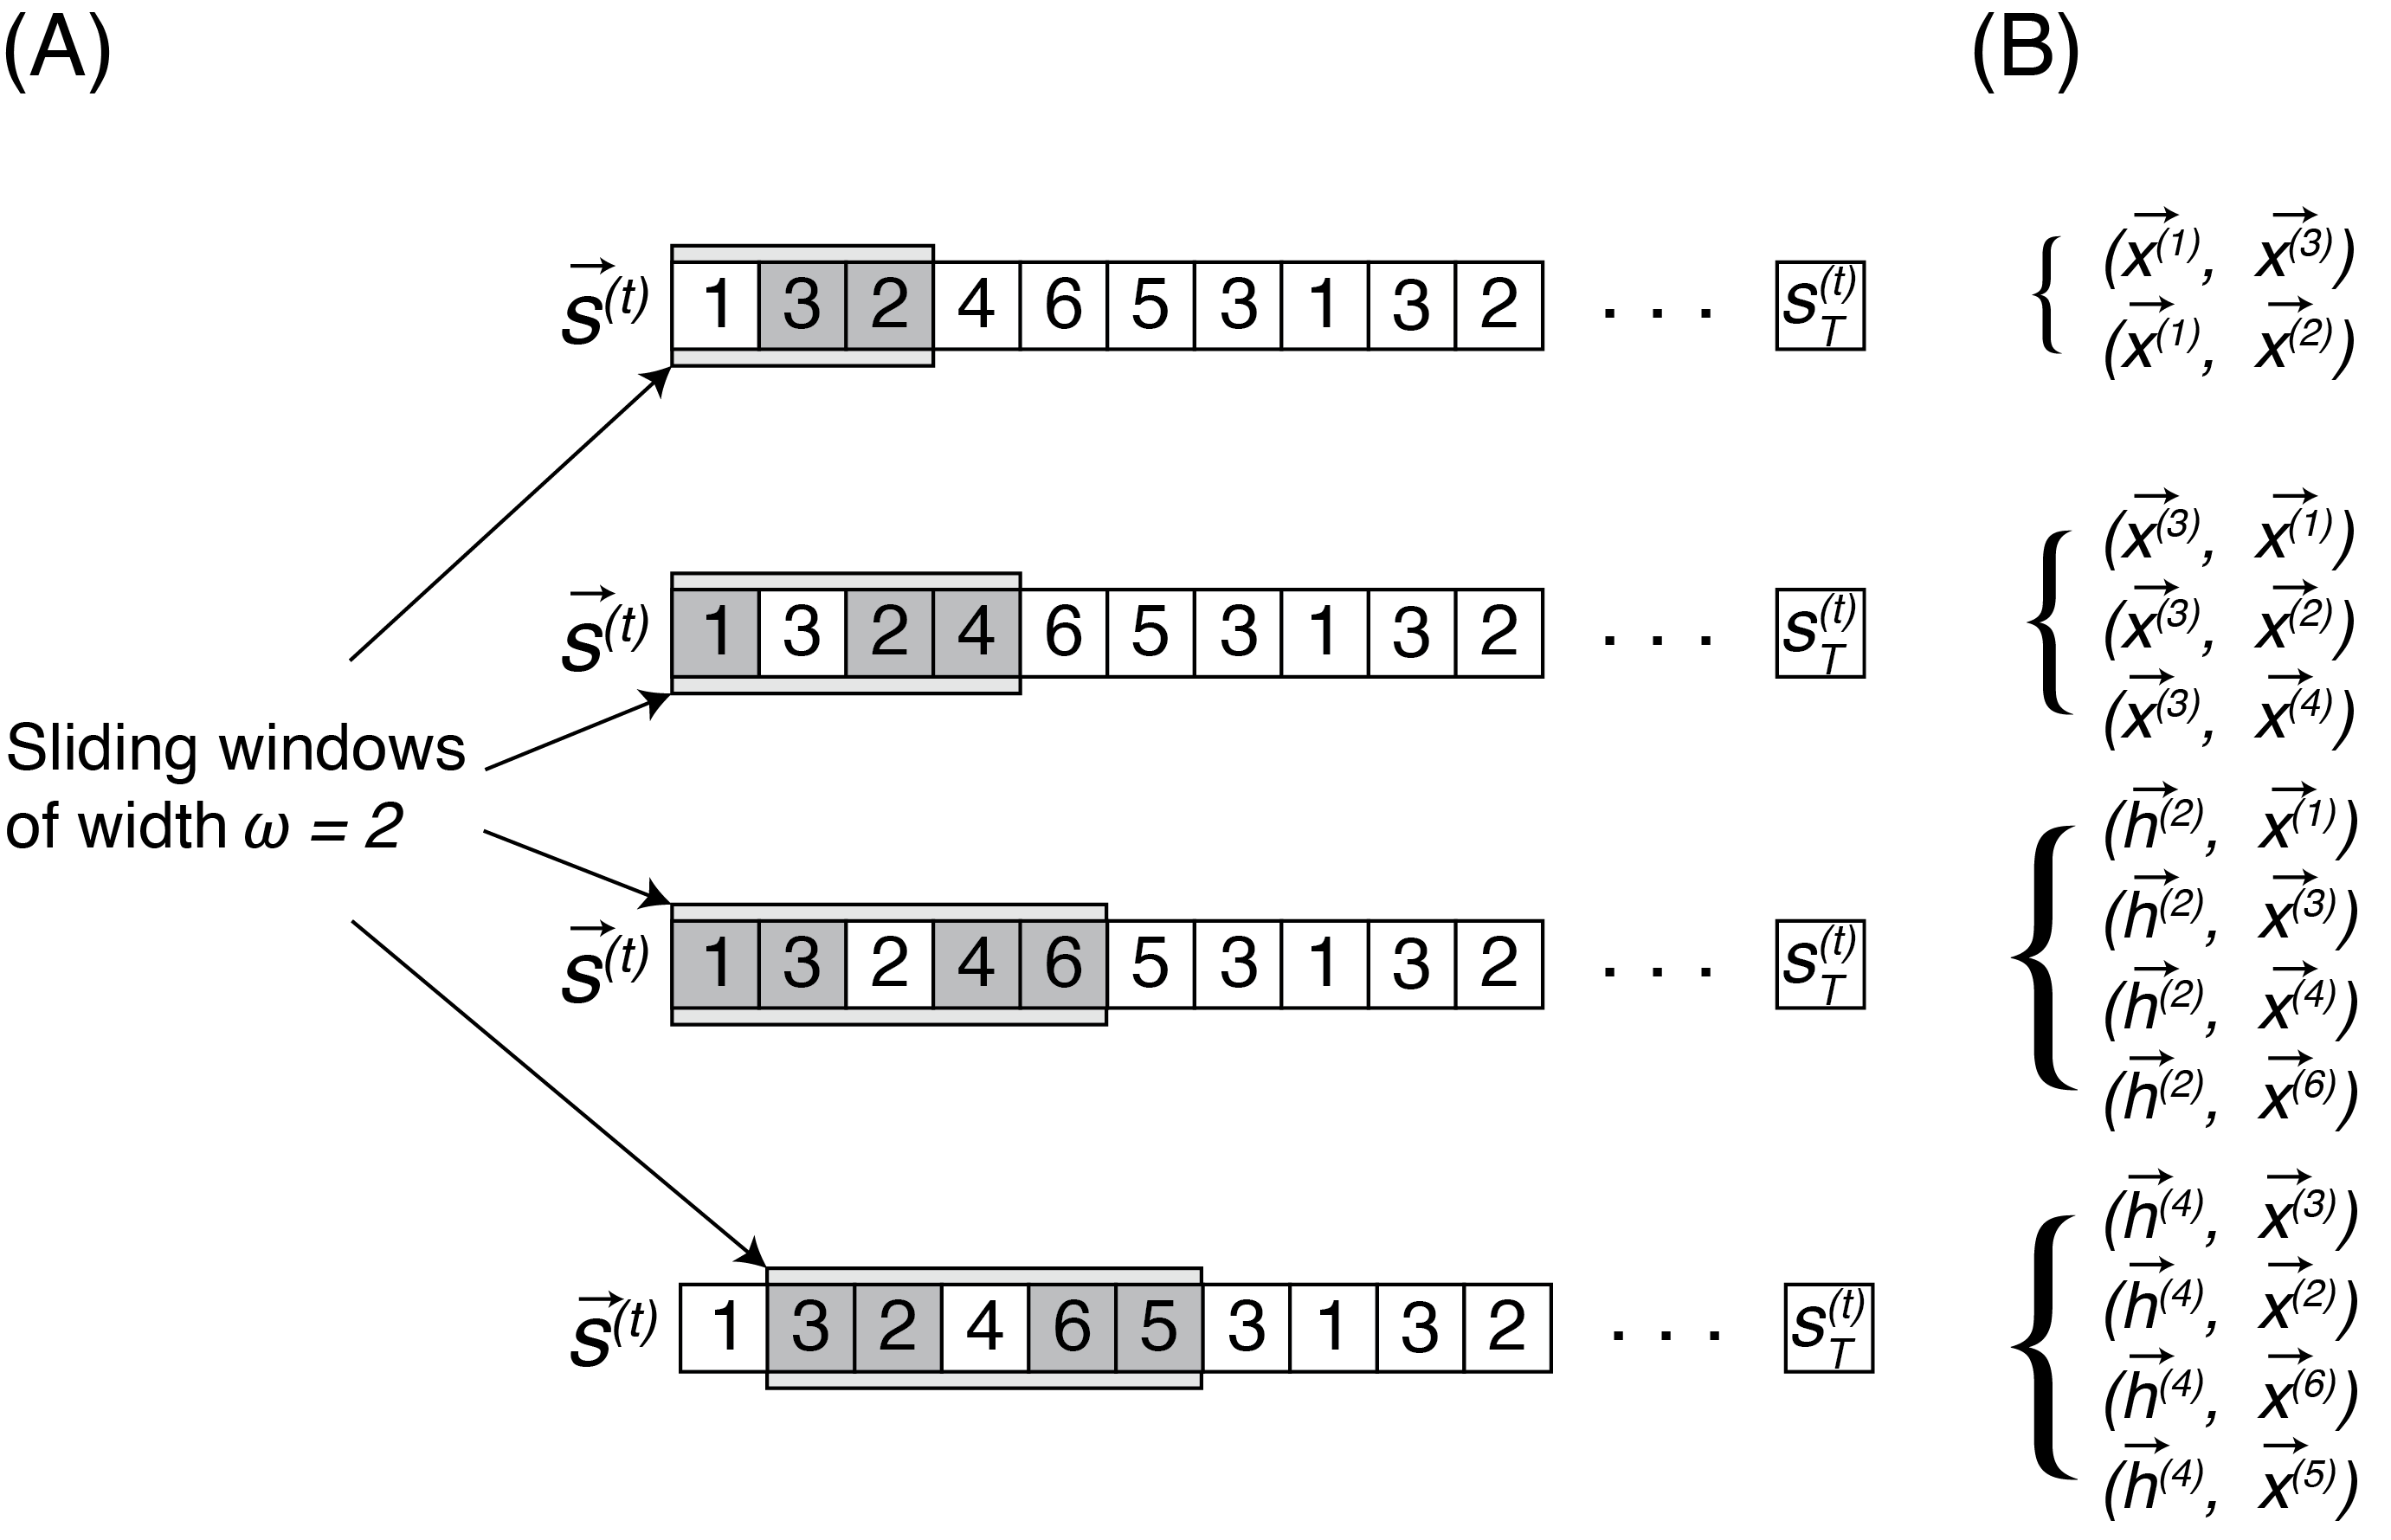
\includegraphics[width=\linewidth]{next/Images/window.png}
    \caption[Computing probability of two nodes being close]{\textbf{(A)} sliding windows moving over a generated random walk, \textbf{(B)} training sample pairs which are generated from the window.}
    \label{fig:next:diff:sliding_window}
\end{figure}

In Figure \ref{fig:next:diff:sliding_window}(B), we illustrate the center nodes and context nodes that will form the training set for our NN. In this case, the center node's one-hot encoding $\vec x^{(i)}$ will be the input to the NN, and the context node's one-hot encoding $\vec x^{(j)}$ will be the expected output for the NN. Together, these form a sample $\left(\vec x^{(i)}, \vec x^{(j)}\right)$.

As we did previously in Section \ref{sec:ch10:gnns}, we split all of these samples into a training and a testing set, and we further randomly reorder the training set into $R$ epochs, each of which contain every training sample (but in a random order). This is illustrated in Figure \ref{fig:next:gnn:training}.

\paragraph*{Defining the learning problem}

For our learning problem, what we want to do is effectively learn the context given the center node. The idea here is that for each training sample, we will use the center of the sliding window $\vec x^{(i)}$ to produce estimated probability vectors $\hat{\vec p}^{(i)}$ that are $n$-dimensional, with a single entry for each possible node in the network. 

If our procedure is successful, the probabilities of context nodes (from our training samples) about a given center node will be higher than the probabilities of non-context nodes about a given center node. For our cost function, we'll minimize the cross-entropy loss between the context nodes (from the training samples) and the predictions (produced by our network). We will denote this loss function by $L(\theta)$, for the parameters $\theta$ for our NN. 

\begin{align*}
    L(\theta) &= -\sum_{i=1}^{N}\vec y^{(i)} \cdot \log(\hat{\vec p}^{(i)})
\end{align*}

In the equation above, N is the number of training samples, $\vec y^{(i)}$ is the true probability vector of the context for the $i^{th}$ sample (usually this is a one-hot vector representing the actual context node), and $$\hat{\vec p}^{(i)}$$ is the estimated probability vector output by your neural network for the i-th sample. The $\log$ function applies element-wise to the vector $\hat{\vec p}^{(i)}.$

This loss function sums the cross-entropy loss over all training samples, and the goal of learning is to adjust the parameters $\theta$ to minimize this sum.

% @AL
% Cross-entropy is a good choice for the following reason. For a series of coin flips, we can estimate the probability the coins land on heads by the fraction of coin flips that land on heads. This is a maximum likelihood estimator. In our case, if we place some assumptions on our training data (the samples generated from the windows), a set of probability estimates which achieve minimum cross-entropy loss are also a maximum likelihood estimator \cite{goodfellow2016deep}.

% https://towardsdatascience.com/word2vec-out-of-the-black-box-a404b4119681
% https://www.youtube.com/watch?v=ERibwqs9p38&ab_channel=StanfordUniversitySchoolofEngineering
% https://medium.com/@corymaklin/word2vec-skip-gram-904775613b4c
% https://www.youtube.com/watch?v=FVv40qv7Dag&ab_channel=KasperGreenLarsen

\paragraph*{Architecture of the network}

The network architecture for the skip-gram model is shown in Figure \ref{fig:next:diff:skipgram}. The first step in Figure \ref{fig:next:diff:skipgram}(A) is the input, which as we discussed previously, is the one-hot encoding for a center node of a given window in a random walk, which we will denote by $i$. In the Figure, we illustrate the one-hot encoding for node $1$ in the network. For each possible center node $i$ in the network, a set of weights $w^{(i)}_u$ connects the node $i$ to hidden layer $u$, for each of the $d$ hidden layers in the network. The number of hidden nodes is the number of ``embedding dimensions'' for the \texttt{word2vec} technique. This is illustrated in Figure \ref{fig:next:diff:skipgram}(B). For each node, this gives us an associated $d$-dimensional vector of weights:
\begin{align*}
    \vec w^{(i)} = \begin{bmatrix}
        w^{(i)}_1 & \hdots &  w^{(i)}_d
    \end{bmatrix}^\top
\end{align*}
Where $d$ is the number of nodes in the hidden layer.

\begin{figure}
    \centering
    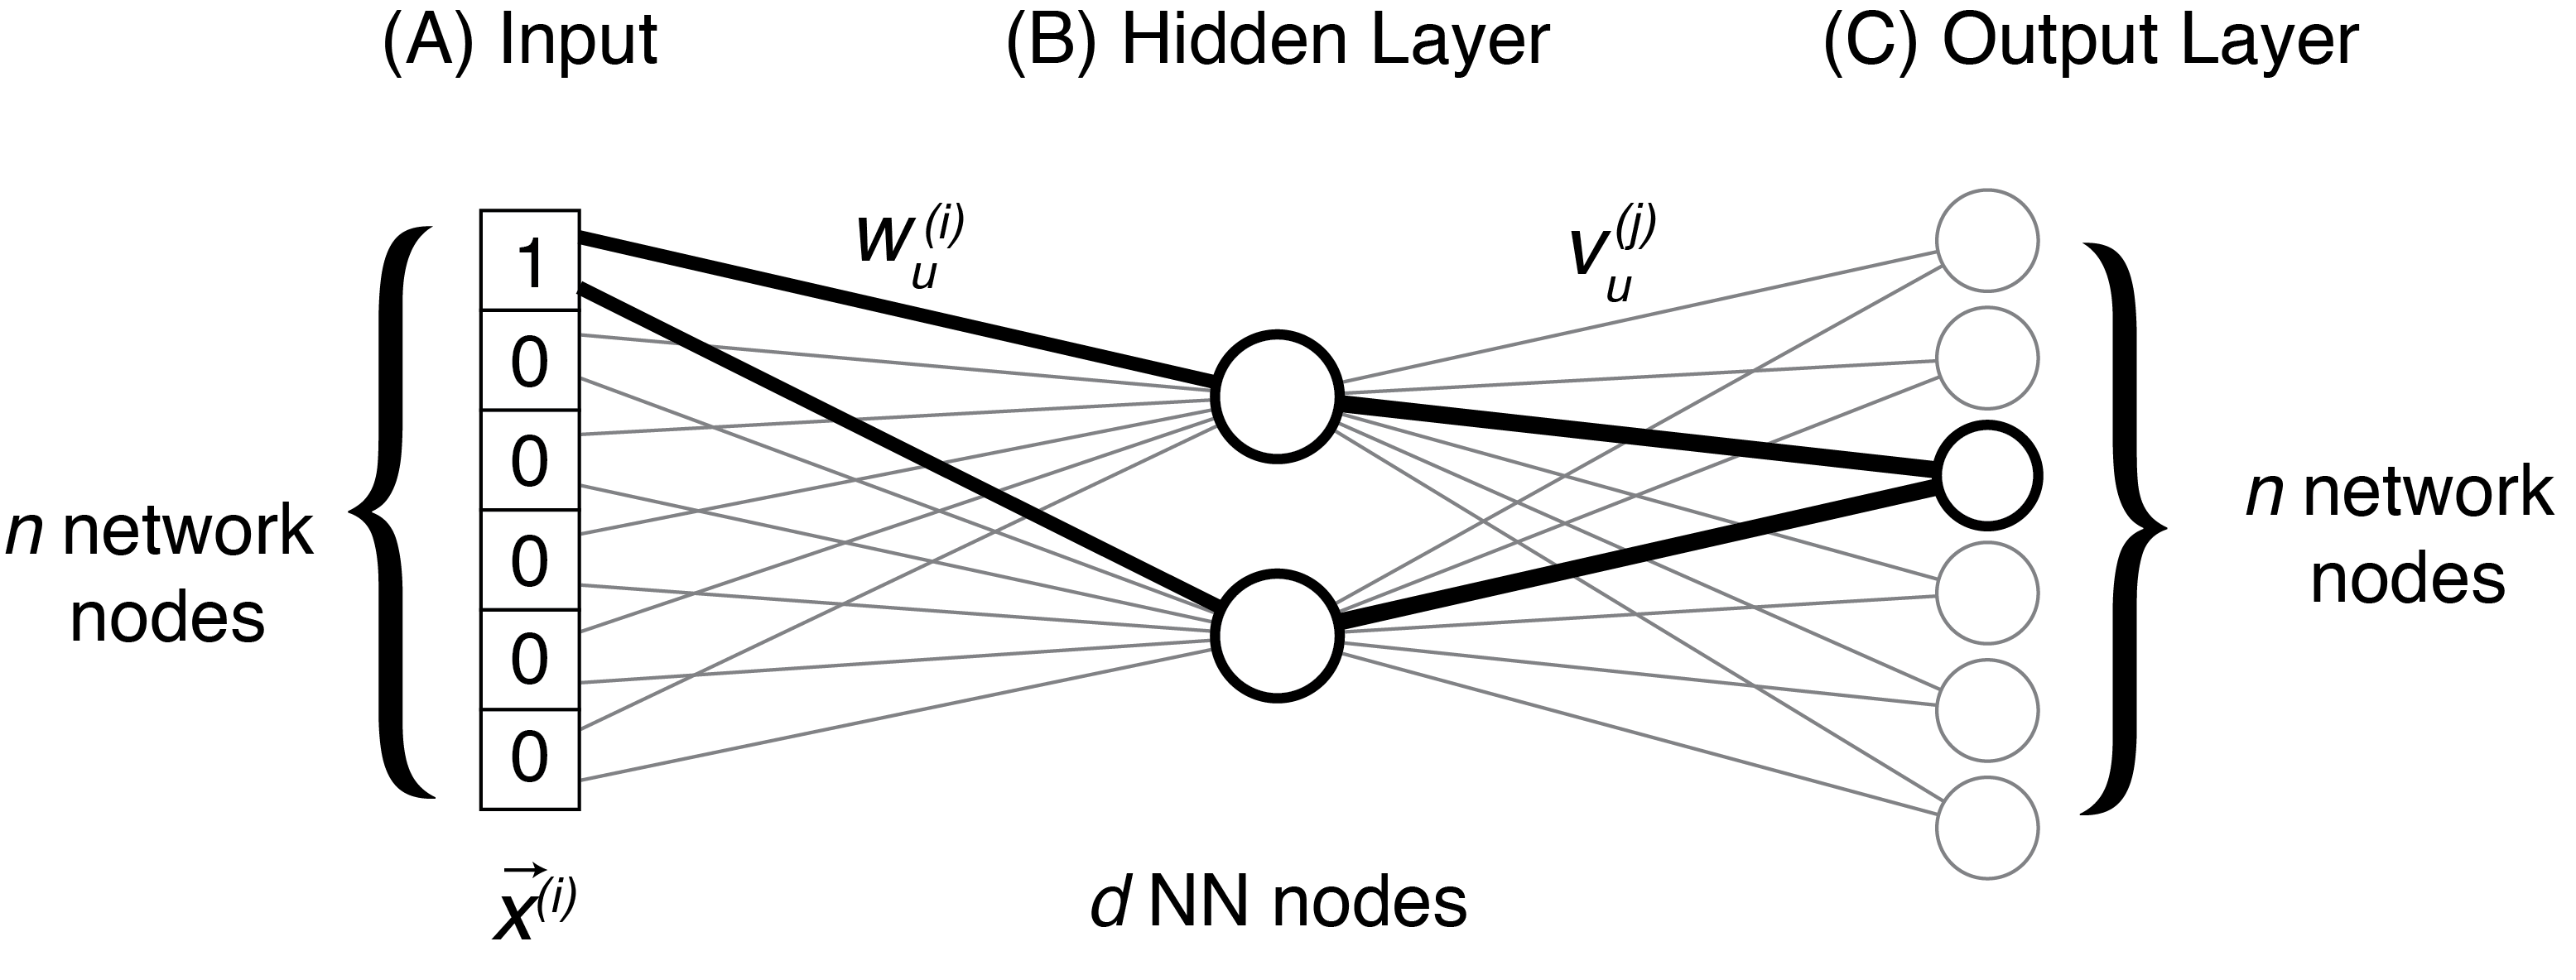
\includegraphics[width=\linewidth]{next/Images/skipgram.png}
    \caption[Skip-gram model]{\textbf{(A)} the input to the network, \textbf{(B)} the hidden layer with $d$ hidden NN nodes, \textbf{(C)} the output layer.}
    \label{fig:next:diff:skipgram}
\end{figure}

These weights are captured in the weight matrix $W$, which has a single row for each possible node in the network:
\begin{align*}
    W &= \begin{bmatrix}
        \leftarrow & \vec w^{(1)}^\top & \rightarrow \\
        & \vdots & \\
        \leftarrow & \vec w^{(n)}^\top & \rightarrow
    \end{bmatrix}
\end{align*}
By pre-multiplying the one-hot encoding vector $\vec x^{(i)}$ by the transpose of this weight matrix $W$, notice that:
\begin{align*}
    W^\top \vec x^{(i)} &= \sum_{j = 1}^n x^{(i)}_j\vec w^{(j)}, \\
    &= \vec w^{(i)},
\end{align*}
which is because $x^{(i)}_j$ is $0$ for any $j \neq i$ (it is a one-hot encoding of node $i$), and $1$ exactly where $j = i$. Therefore, we obtain the row of weights corresponding to the node $i$. The idea here is that we are using the weights connecting the input and hidden layers to define a latent representation of the node $i$, which is the vector $\vec w^{(i)}$.

Finally, the output layer has $n$ nodes, one for each node in the network, illustrated in Figure \ref{fig:next:diff:skipgram}(C). The set of output weights $v_{u}^{(j)}$ connect the hidden node $u$ to the output node $j$. With the hidden layers as the rows and the outputs as the columns, this produces a $d \times n$ matrix $V$ for us, with columns $\vec v^{(j)}$ for each node in the network. The probability that a node $i$ has a node $j$ at least $\omega$ close (the window width) is modeled using the equation below:

\begin{align*}
    p^{(i)}_j = \sigma\left(V^\top\vec w^{(i)}\right)_j &= \frac{\exp\left(\vec v^{(j)}^\top \vec w^{(i)}\right)}{\sum_{j' = 1}^n \exp\left( \vec v^{(j')}^\top \vec w^{(i)}\right)}. \numberthis \label{eqn:next:diff:softmax}
\end{align*}

Notice that the exponential function $\exp(\cdot)$ can \textit{only} have positive values for finite inputs, regardless of the product between $\vec v^{(j)}$ and $\vec w^{(i)}$.% Its values are also bounded between 0 and 1, and sum to 1. This makes it useful as a method to turn arbitrary real values into probabilities.
% ^not true for the exponential function, that is only after the normalization by the sum
Therefore, the numerator of the above equation indicates that the weights $\vec w^{(i)}$ and $\vec v^{(j)}$ convey a level of similarity between nodes $i$ and $j$, in that when the value is high, they tend to be within an $\omega$-width window of one another (and therefore, in a similar context). 

Finally, we then normalize this quantity by looking at the other nodes which node $i$ could have been close to in the random walk to produce a probability estimate. This function $\sigma(\cdot)$ is known as the \textit{softmax} activation function \cite{goodfellow2016deep}, commonly used in the output layer for neural networks which predict probabilities of sets of different outcomes. Here, we have $n$ possible outcomes that we are predicting (whether a given node $j$ is a context node for center node $i$, where nodes $j$ range from $1$ to $n$). 

Conceptually, the quantity $\sigma\left(\vec w^{(i)}^\top V\right)_j$ can be thought of as an estimate of the probability of the context being node $j$ given that node $i$ is the center node, and is denoted by $p^{(i)}_j$. The vector $\vec p^{(i)}$ is a length $n$ vector, whose entries $p^{(i)}_j$ denote the probability of node $j$ being contexts for center node $i$:

\begin{align*}
    \vec p^{(i)} &= \begin{bmatrix}
        p^{(i)}_1 & \hdots & p^{(i)}_n
    \end{bmatrix}^\top.
\end{align*}

In total, the parameters $\theta$ for our NN are the two weight matrices, denoted by the set $\left\{W, V\right\}$.

\paragraph*{Training the network}

As in Section \ref{sec:ch10:gnns}, we split the samples produced by Figure \ref{fig:next:diff:sliding_window}(B) into training and testing sets, reorder the elements of the training set into epochs (where each epoch contains each training sample, but in a different order), and then split the epochs into $B$ batches.

For a given parameter set $\theta = \left\{W, V\right\}$, we feed a batch of training samples through the network one at a time, as indicated in Figure \ref{fig:next:diff:sgtraining}. To recap, this procedure was:
\begin{enumerate}
    \item Compute the one-hot encoding of center node $i$, as $\vec x^{(i)}$.
    \item Obtain the $i^{th}$ row of the weight matrix $W$, by taking $\vec w^{(i)} = W^\top \vec x^{(i)}$.
    \item Predict probabilities for each possible output node $j$ being a context node for $i$, with $p^{(i)}_j = \sigma\left(V^\top \vec w^{(i)}\right)_j$, according to Equation \eqref{eqn:next:diff:softmax}.
\end{enumerate}

\begin{figure}
    \centering
    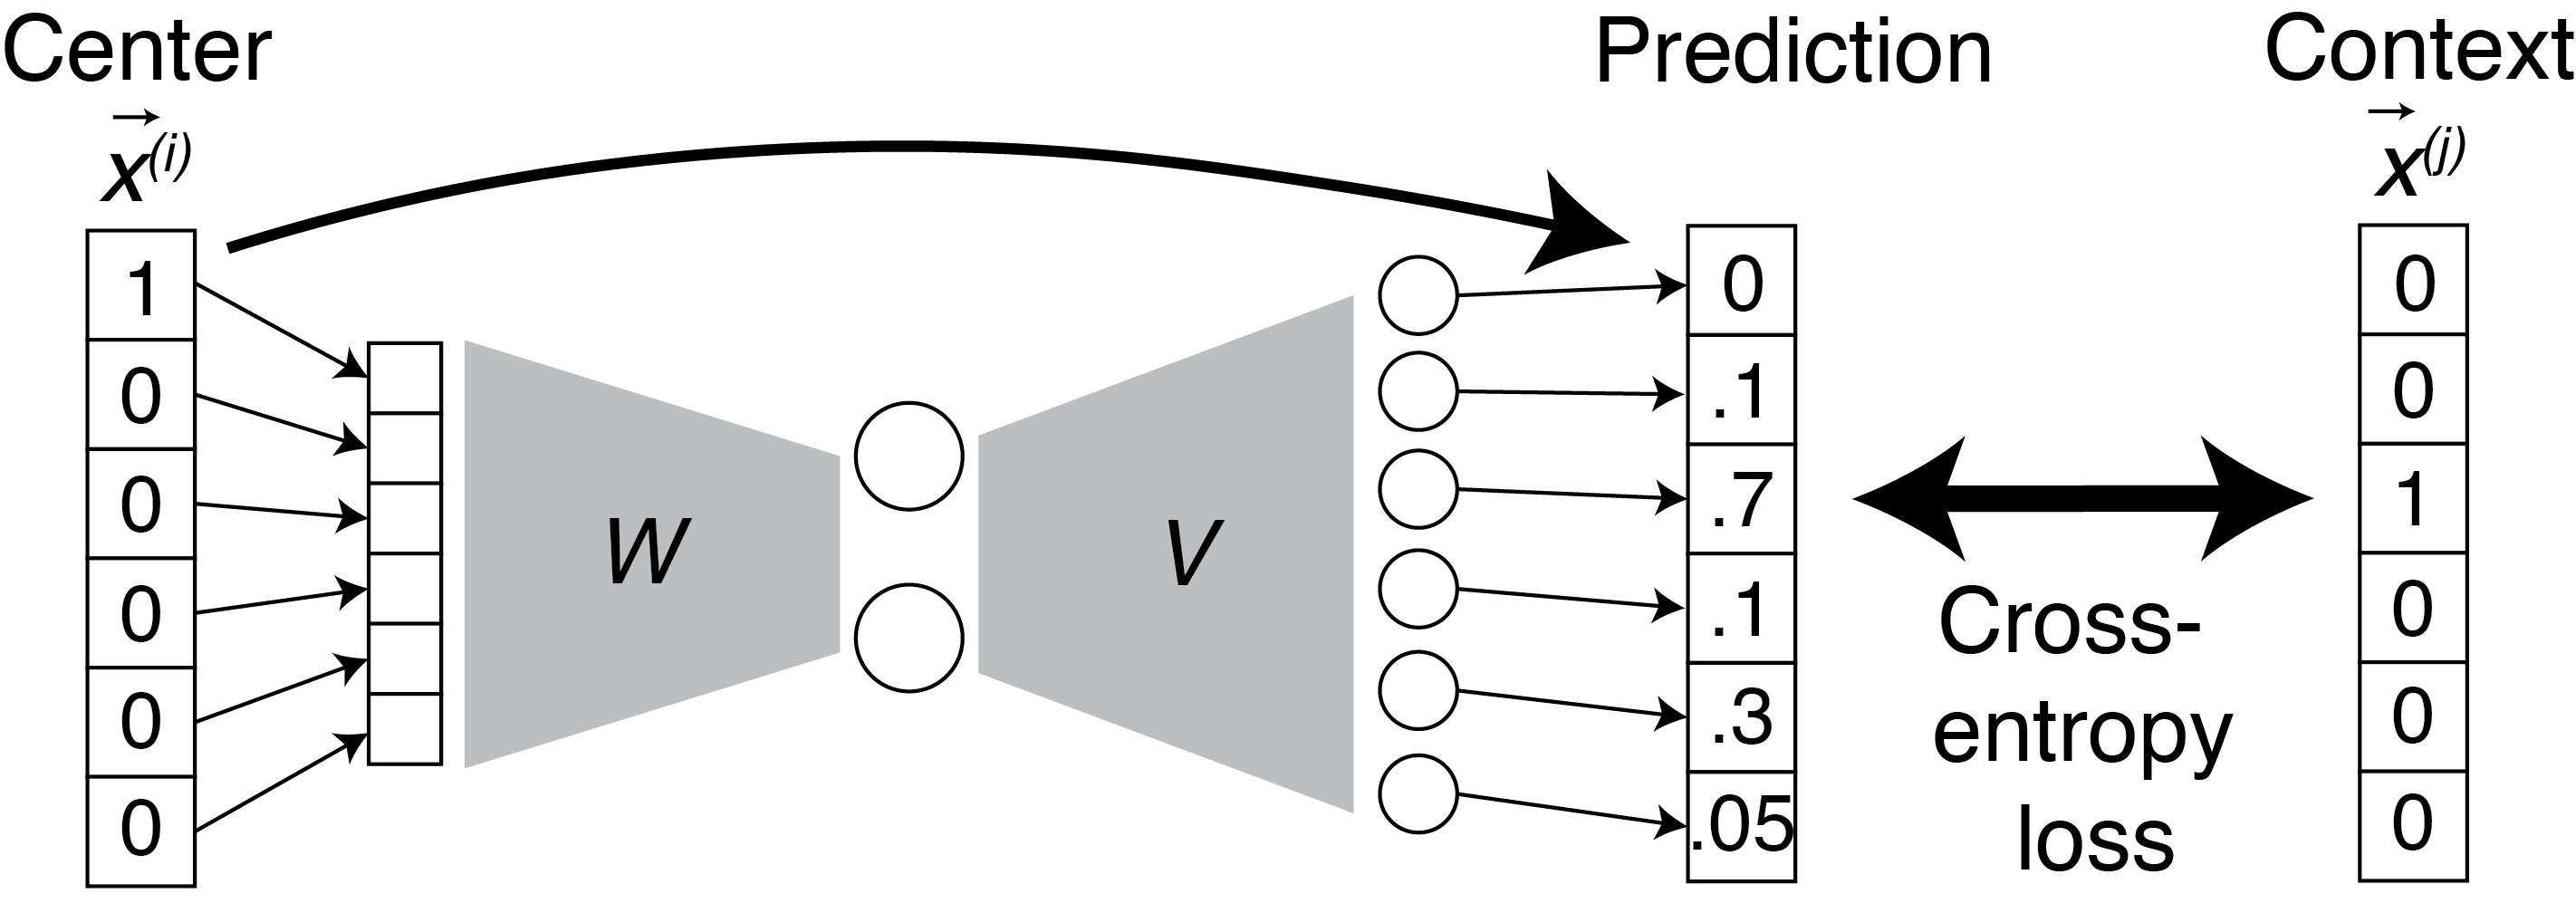
\includegraphics[width=\linewidth]{next/Images/skipgram_forward.png}
    \caption[Forwards pass through a skip-gram network.]{A forwards pass through a skip-gram network for a single training example, with a center node $i$ and a context node $j$}.
    \label{fig:next:diff:sgtraining}
\end{figure}

This procedure gives us a probability vector $\vec p^{(i)}$. We repeat this process across an entire batch.

The next ingredients that we need are the gradients of the loss function $L(\theta)$ with respect to the weight matrices $W$ and $V$. This quantity can be written as $\nabla_{W, V} L(W, V)$, which has entries of the form $\frac{\partial L(W, V)}{\partial w_{ik}}$ or $\frac{\partial L(W, V)}{\partial v_{kj}}$ for each node $i$ and $j$, and each embedding dimension $k$. As we discussed in Figure \ref{fig:ch8:gm:grad_desc} and Section \ref{sec:ch10:diffusion}, these gradients indicate how the loss $L(W, V)$ will change when we alter the matrix parameters $W$ and $V$ of our NN for each entry. We make a backwards pass using gradient descent to update these existing weight matrices to form $W'$ and $V'$, as in Figure \ref{fig:next:gnn:epoch_compute}. We repeat this procedure for all batches in our epoch. For a technical discussion on how to perform gradient descent, see \cite{goodfellow2016deep}.

\begin{floatingbox}\caption{Concept: implementation}
    In practice, there are python libraries that do this already; if you want to write it up by hand, you should use one of the many deep learning frameworks; pytorch would be a great start.
\end{floatingbox}

When we finish off the epoch, we compute the cross-entropy loss on the held-out testing samples. We repeat this process over and over again for each epoch, until we reach our stopping criterion (which is typically convergence of the cross-entropy loss on the held-out testing samples).

For a more technical discussion on the mathematics behind the skip-gram model, check out \cite{PourNejatian2021Dec}.

\paragraph*{Obtaining an embedding from the skip-gram model}

After all of that work, you will be surprised with just how simple obtaining an embedding from \texttt{word2vec} is for our nodes. We simply take the weight matrix $W$, which has $n$ rows and $d$ columns, and use each row $\vec w^{(i)}$ as the embedding for node $i$. Nodes which tend to be along random walks together tend to end up closer in the embedding space, and nodes which do not tend to be along random walks together tend to end up further in the embedding space. 

Conceptually, if two nodes tend to fall along similar positions in random walks, it would be desirable if their predicted context nodes were similar, which were computed from $\vec p^{(i)} = \sigma\left(V\vec w^{(i)}\right)$ for a given node $i$. This is because if, say, node $2$ tends to fall in a similar context to node $1$, and node $3$ tends to occur in a similar context to node $2$, it is quite likely that node $3$ and node $1$ also fall into similar contexts. This is due to the fact that \textit{context}, in this case, was enforced using a window of fixed width $\omega$, which means that nodes $1$ and $2$ which share a similar context (and are within a window of one another) will necessarily have a subset of nodes (falling between the two) that are in each of their contexts. Since $V$ is fixed for any given center node $i$, the only way that this can be the case is if the word embeddings $\vec w^{(i)}$ are similar to an extent, which illustrates that this procedure conceptually satisfies our original aim.

\begin{floatingbox}\caption{Concept: using NNs and GNNs to obtain latent embeddings}
This section illustrates a potent use-case for neural networks. As we discussed in Section \ref{sec:ch10:gnns}, neural networks and GNNs applied to network data that are structured typically perform an ``embedding'' step of some form, whether it is explicitly or implicitly incorporated into the architecture. 

To obtain a latent embedding, we can simply ``remove'' sets of layers of the NN, and learn about the network using the latent representation learned in the preceding layers. In this section, we illustrate that by just ignoring the output softmax layer, we can obtain the \texttt{node2vec} embedding of the network. In some sense, these successive layers existed solely so that the preceding layers would be part of a sensible learning task that we could apply to the network. 
\end{floatingbox}

\subsubsection*{Using \texttt{node2vec} with network data}

To illustrate the utility of \texttt{node2vec}, we will construct an example that is a little bit different from what we are used to. We will use a $4$-community $SBM$, where the block matrix has both affinity and core-periphery structure, from Section \ref{sec:ch5:psd_block}. The idea here is that there are two ``communities'' of nodes which have higher within-community probabilities than between-community probabilities, and within each community there are ``sub-communities'' which have higher average node degrees (the core) and lower avererage node degrees (the periphery):

\begin{lstlisting}[style=python]
from graphbook_code import dcsbm

nk = 50  # 50 nodes per community
zs = np.repeat([1, 2], 50)
B = np.array([[0.6, 0.2], [0.2, 0.6]])  # same probabilities as from SBM section
theta = b = np.repeat([1, .5, 1, .5], 25)
deg_map = {1: "Core", 0.5: "Per."}

zs_aug = ["{:d}, {:s}".format(z, deg_map[theta[i]]) for i, z in enumerate(zs)]
A, P = dcsbm(z, theta, B, return_prob=True)
\end{lstlisting}

\begin{figure}
    \centering
    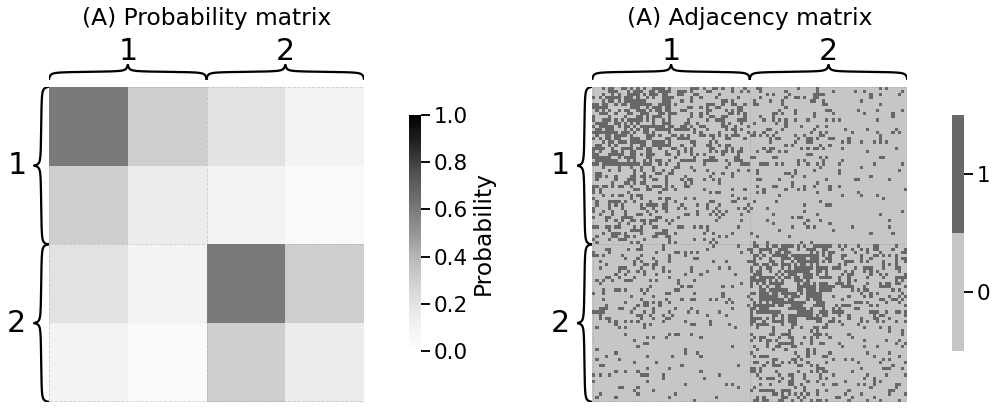
\includegraphics[width=0.8\linewidth]{next/Images/diff_ex.png}
    \caption[Example for \texttt{node2vec}]{\textbf{(A)} the probability matrix for our network, \textbf{(B)} a realization of our network.}
    \label{fig:next:diff:ex}
\end{figure}

We show the probability matrix and a realization in Figure \ref{fig:next:diff:ex}(A) and Figure \ref{fig:next:diff:ex}(B), respectively.

Let's try embedding this example using \texttt{node2vec}. We're going to leave the in-out and return parameters both equal to one, for now; e.g., $p = q = 1$. In this case, the second-order biased random walk is equivalent to a first-order walk, since $p = q = 1$. This is because the biases all turn out to be one, so the ``bias factors’’ turn out to really just be the first-order transition probabilities from the normal random walk. So why do we want the flexibility of the second-order biased random walk, if we can embed our network using the first-order random walk?

We will generate $20$ random walks starting at each node ($r = 20$), each walk will have a length of $200$ steps ($T = 200$), and :

\begin{lstlisting}[style=python]

\end{lstlisting}

Which is illustrated as a pairs plot in Figure \ref{fig:next:diff:embed}(A) along with the true (unknown) community labels. 

\begin{figure}
    \centering
    \includegraphics{}
    \caption{\textbf{(A)} A pairs plot of the \texttt{node2vec} embedding with $p=q=1$, \textbf{(B)} A pairs plot of the \texttt{node2vec} embedding with $q = 5$, $p = \frac{1}{5}$.}
    \label{fig:next:diff:embed}
\end{figure}
\subsubsection*{What utility is added by a second-order biased random walk?}

The reason we leverage second-order biased random walks is that they give us flexibility. You will notice that since the \texttt{node2vec} procedure relies on the ``corpus'' of random walks, that the behavior of these random walks will have a substantial influence on the resulting embedding. Let's see what happens to our embeddings as we tend to favor moving within the same nodes for our random walks more, which means punishing in-out movements ($q$ is larger, so let's use $q=5$) and up-weighting return movements ($p$ is smaller, so let's use $p = 0.2$):

\begin{lstlisting}[style=python]
\end{lstlisting}

Which is illustrated as a pairs plot in Figure \ref{fig:next:diff:embed}(B) along with the true (unknown) community labels. 

It looks like dimensions one and two do a great job of capturing the differences between $C1$ and $C2$ nodes. 


Simultaneously, when we remember that the \texttt{node2vec} algorithm builds off the idea of the \texttt{word2vec} algorithm at preserving nodes which have a similar ``context'', we know that the core nodes all share a similar context (they are more strongly connected) than the peripheral nodes (which are less strongly connected). Note that the ``core'' nodes are all at the ``core'' of the third and fourth embedding dimensions, and the ``periphery'' nodes are all at the ``periphery'' of the third and fourth embedding dimensions.

Toying around further with these different parameters can yield us very different ways to represent the same network in Euclidean space.

\subsection{Extending to weighted or directed networks}

It is extremely easy to adapt the strategies we have developed so far to weighted or directed networks. If the network takes non-negative weights, and the weights $w_{ij}$ can be interpreted to indicate the ``strength’’ of a connection between a node $i$ and $j$, we can just let the transition probabilities $p_{ij}$ be the weights normalized by the out-degree from node $i$; that is:
\begin{align*}
    p_{ij} &= \frac{w_{ij}}{d_i}
\end{align*}
where the out-degree is the quantity $d_i = \sum_{j = 1}^n w_{ij}$.